\documentclass[12pt,twocolumn]{article}



%\usepackage[utf8]{inputenc}
\usepackage{amsmath}
%\usepackage{ae}
\usepackage{graphicx}
\usepackage{color}
\usepackage{bbm}
\usepackage[swedish]{babel}
\newcommand{\N}{\ensuremath{\mathbbm{N}}}
\newcommand{\Z}{\ensuremath{\mathbbm{Z}}}
\newcommand{\Q}{\ensuremath{\mathbbm{Q}}}
\newcommand{\R}{\ensuremath{\mathbbm{R}}}
\newcommand{\C}{\ensuremath{\mathbbm{C}}}
\newcommand{\rd}{\ensuremath{\mathrm{d}}}
\newcommand{\id}{\ensuremath{\,\rd}}
\newcommand{\ket}[1]{|#1\rangle}
\newcommand{\bra}[1]{\langle#1|}
\newcommand{\braket}[2]{\bra{#1}#2\rangle}
\newcommand{\bracket}[3]{\bra{#1}#2\ket{#3}}

\title{adsf}
\author{}
\newpage

\begin{document}
\tableofcontents
\renewcommand{\abstractname}{Abstract}
\begin{abstract}
\end{abstract}
\section{Introduction}

\section{Experimental setup}
In this experiment we used two plastic scintillator detectors located on top of each other with a gap of 2.4 meters. Below the lowest one we also had a barrel. See fig(). When a muon goes through one of the scintillator detectors we will get a pulse that is amplified by a photo multiplier. By then measuring the time difference between pulses from respective detector we can determine the speed of the muons. We also placed a radiactive $^{60}$Co sample below the lowest detector for calibration, since it releases two photons at the same time and we can thus capture the event when the photons gets absorbed in different detectors. The pulses from the two detectors were delayed in such a way that these two measurements could be done at the same time.\newline

To determine the lifetime of the muons we used on scintillator and the barrel detector. Coincidence between the barrel and the scintillator were used to be able to identify signals from muons that went through the scintillator and then absorbed in the barrel. The barrel will first give a signal from the energy absorbed when slowing down the muon and another signal when it decays. The start and stop signals are separated by an AND respectively AND-NOT gate with the scintillator signal, see fig().



\section{Results}



\section{Conclusions}


% Figurer inkluderade som eps-filer
%% \begin{figure}\centering
%% 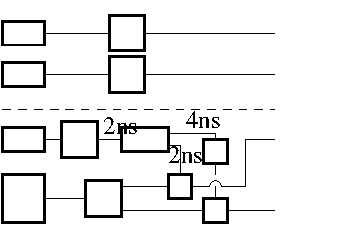
\includegraphics{speed.pdf}
%% \caption{\label{figuren} Perioden $T$ som funktion av pendellängden.}
%% \end{figure}

% Figurer inkluderade med xfigs postscript+latex

\begin{figure}[h]
\input{speed.pspdftex}
\caption{\label{setup} Schematic diagram of the different operations acting on the input signals.}
\end{figure}

\end{document}
